\documentclass[11pt,letterpaper]{article}
\oddsidemargin 0in
\evensidemargin 0in
\textwidth 6.5in
\topmargin -0.5in
\textheight 9.0in
\usepackage{hyperref}
\usepackage{mathptmx}
\usepackage{graphicx}
\usepackage{amsmath}
\usepackage{relsize}
\usepackage{natbib} % for references
\usepackage[usenames,dvipsnames]{xcolor}
\newcommand{\blue}[1]{\textcolor{RoyalBlue}{#1}}
\newcommand{\fillme}[1]{\blue{\texttt{[Insert #1]}}}
\newcommand{\instructions}[1]{\blue{\textit{#1}}}

\begin{document}

\title{CS446 Class Project - Stockit}
\author{dmcquil2@illinois.edu, mcconne7@illinois.edu}
\maketitle



%\instructions{If you are taking CS446 for 4 hours credit, you need to do a research project. This is a template for the project report that you need to hand in at the end of the semester, but it should also help you guide you as you work on the project. In particular, you should work on the Introduction, Background, Task and Data sections before you perform any experiments yourself. Note that you cannot perform any machine learning experiments without having suitable test and training data, or knowing what to evaluate.}

\begin{abstract}
%\instructions{Very briefly, summarize your task, your model and your main results}
Stockit is a machine learning algorithm that forecasts a single stock price movement
from the content of a news article.
\end{abstract}

\section{Introduction}
\label{sec:introduction}
%\instructions{This should be a brief outline of the paper -- use plain English, no math. Note that you should be able to write most of this section before you actually perform any experiments. First, define and motivate your task: what are you trying to learn, and why is this an important task? Second, define what kind of a machine learning problem this requires you to solve (binary/multiclass classification, ranking, ....). What is an appropriate baseline model for this task? What kind of model are you proposing? 
%Briefly summarize the assumptions your model makes. Finally, describe the hypotheses you wish to test. These are typically statements of the form ``we expect model/features A to perform better on this task than model/features B''.
%Outline how your experiments will evaluate these hypotheses (comparisons of different models, ablation studies, learning curves, oracle experiments... ). }
We created an algorithm that forecasts a stock price movement from news
article content and historic stock prices.
We pursued this algorithm because it's prediction could act as an indicator to
whether a stock is about to increase or decrease in price. We used a
text search algorithm to rank the tickers on document relevance. Then we created
a kNN implementation to cluster the documents according to a positive or
negative price movement in the mentioned stock. \\  \\
We propose a model that will predict the stock price movement focused around
document similarity and clustering.
Two variations of this model will be tested:
\begin{itemize}
	\item A model with using the arithmetic mean of its kNN neighbors. This will
    require a base feature set of the percentage change for each document.
	\item A probabilistic model uses the similarity between documents as a
    probability measure. It will use this probability to calculate the expectation of
    the stock price movement. This will require both the
    base feature set of the percentage change of a document as well
    as the similarity score between the queried document and the sorted retrieved documents.
\end{itemize}
We expect the model with the calculated probability to perform better than
the model that is uniformly distributed. Our hypotheses will be evaluated
against results from a purely regressive model. ~\cite{arizona}\\ \\
Ultimately, we would like to prove that calculating stock trends using news
articles is more accurate than observing the stocks history.

\section{Background}
\label{sec:background}
%\instructions{Summarize and discuss related work that you are building on: this requires you to find, read and cite a few research papers. This is also something you can get started on as soon as you have settled on a task.} 
There have been other attempts to predict stock market prices using machine
learning. For example, \href{http://ailab.arizona.edu/intranet/papers/Textual\%20Analysis\%20of\%20Stock\%20Market.pdf}{Textual Analysis of Stock Market Prediction Using Financial News Articles}
approaches this challenge from a very similar direction. Their research has
shown that text information can provide a 1\% to 2\% increase in accuracy of
predicting the change in a stock price than a purely regressive model ~\cite{arizona}

\section{Task and Data}
\label{sec:taskAndData}
%\instructions{Now describe the task and data in more detail.}

\subsection{The Task}
\label{sec:task}
%\instructions{Now, try to formalize your task as a classification/ranking/... problem. Introduce mathematical/formal notation as necessary. How do you evaluate models, or measure success?}
In order to predict stock trends we will be using a k nearest neighbor
algorithm that will cluster the documents. This algorithm will
first generate a similarity score for all documents.
The similarity between documents will be calculated using the
following similarity function. ~\cite{similarity}
\begin{equation}\label{doc:sim}
	sim(d_i, d_j) = coord(d_i, d_j) \cdot queryNorm(d_i) \cdot \Sigma_{t \in d_i} \left[ tf(t \in d_j) \cdot idf(t)^2 \cdot norm(t,d_j) \right]
\end{equation}
where
\begin{description}
	\item[\(tf(t \in d_j)\)] : this is the term frequency of a term in document \(d_j\) where \(t\) is a term present in document \(d_i\)
	\item[\(idf(t)\)] : this is the inverse document frequency for a given term in a document as defined as
	\begin{equation}\label{doc:idf}
		idf(t) = 1 + \log \left[ \frac{numDocs}{docFreq(t) + 1} \right]
	\end{equation}
	\item[\(coord(q,d_j)\)] : this is a score based on how many of the query terms are found in a given document \(d_j\)
	\begin{equation}\label{doc:coord}
		coord(q,d_j) = \frac{\text{\# of query terms found in } d_j }{\text{\# of query terms}}
	\end{equation}
\end{description}

\begin{description}
	\item[KNN] : We implement KNN using the text similarity of the document to
    find its nearest neighbors and record the percentage changes of the stock referenced.
  \item[Constraints] :
    \begin{itemize}
      \item We make sure to only use neighbors which are included in the training data.
      \item We make sure the price movement of the stock referenced in the document is calculated
            using the next day's open/close price from the document
            published date. ~\cite{stock-matrix}
    \end{itemize}
\end{description}


\subsection{The Data}
\label{sec:data}
%\instructions{Describe the data you use to train and evaluate your models. Describe where you got it from (include references/citations to published works, or URLs!). Describe and give examples for the features that you have access to.} 
For the purpose of this project we have set up a \href{http://lucene.apache.org/solr/}{solr}
instance to use as our datasource and text computing platform to
handle the large amounts of data. We split our data into three datasets.
This solr instance is currently deployed to \href{http://solr.deepdishdev.com:8983/solr}{solr.deepdishdev.com/solr}. \\ \\
To find relevant articles we were required to search the articles
for a given ticker name and retrieve results whether the ticker
was present or the name of the company. We used a synonyms file generated
from the tickers that were present in the stocks dataset. We also used Porter
stemming ~\cite{porter} to improve search results. \\ \\
Using our three datasets we will create a fourth composite dataset that will
be a document set that contains an article, the most relevant ticker, and
the history for the day following the release of the article. We use a
set of synonyms generated from our stock aliases set.
For a given query and a document we calculate the score using the
similarity function above. \\ \\
\begin{equation}\label{doc:score}
  	score(d_j, d_k) = sim(d_j, d_k)
\end{equation}
where \(V\) is a mapping function that translates both the query and
document to a search vector \\ \\
To find the most relevant ticker we will find the ticker for each
article that has the highest correlated score.  This will give us a new
composite dataset which we will use as our training and test data for our algorithm.
\begin{itemize}
  \item \textbf{Stock history}
  - This dataset will represent the historical stock data going back to 2001
    for all stocks available on Yahoo's financial data
    platform (~24,000 stocks). This historical information was
    retrieved via the \href{https://developer.yahoo.com/yql}{Yahoo data platform}.
\item \textbf{Stocks}
  - This dataset is a listing of all stocks currently available on the
    Yahoo financial data platform including their categories and indexes.
    This index also contains the current aliases for each stock as well.
\item \textbf{News Articles}
  - The dataset is a collection of news articles that have been retrieved
    from various websites using web scraping. Currently this dataset
    consists of content from the following sources:
  \begin{itemize}
    \item \href{http://www.newsmax.com/archives/}{newsmax.com}
  \end{itemize}
\item \textbf{Stock Articles}
  - The dataset is a joined collection of the above three data sets.
    This will be used as our training and testing data for our model.
    Each document in the dataset, D will consist of:
  \begin{description}
    \item[title] : The title of an article
    \item[content] : The contents of a scraped article
    \item[date] : The date that an article was published
    \item[symbol] : The symbol of the stock with the highest correlation to the article
    \item[stockHistoryDate] : The day after the article was released. This
      will be the date for which we will retrieve stock history.
    \item[close] : The closing price of a given stock for the specified date
    \item[open] : The opening price of a given stock for the specified date
  \end{description}
\end{itemize}

\section{The Models}
\label{sec:models}

\subsection{Baseline Models}
\label{sec:baseline-models}
%\instructions{In order to know how difficult the task is and how well we are doing, we need to know how well a suitable baseline model would perform. Define a baseline model for your task. This may not necessarily be a learned model.}
The baseline model we will choose to measure against stockit is a simple random guess.
50\% choose a positive price movement otherwise a negative price movement. This problem is a bit unique
where simply classifying with high accuracy does not guarantee good real world accuracy. It is important that the \\ \\
\begin{equation}\label{acc:constraint}
	\sum_{d}^{D_c} \text{percentageChange}(d) > \sum_{d}^{D_{\text{in}}} \text{percentageChange}(d)
\end{equation}
where
\begin{description}
	\item[\textbf{\(D_c\)}] : The correctly classified documents
	\item[\textbf{\(D_{\text{in}}\)}] The incorrectly classified documents
\end{description}
Note that our model does not take this into effect.

\subsection{Existing Models}
\label{sec:existing-models}
%\instructions{If people have worked on this task before, summarize (and cite) some of the existing models}
One of the baseline models is the linear regression model. The prediction for a stock is given by
\begin{equation}\label{pred:uniform}
	\text{prediction}(s, i) = \mathlarger{ \mathlarger{ \sum } }_{i=i}^{n} \frac{\text{percentageChange}(s, \text{day}_i) }{ n }
\end{equation}
where \begin{description}
	\item[\textbf{s}] : A given stock in the set S which represents the set of all stocks in our dataset
	\item[\textbf{\(\text{day}_i\)}] : A historic day for a given stock \(S\)
	\item[\textbf{n}] : The total number of days
\end{description}
One paper created a model by using text mining with sparse matrix factorization.~\cite{stock-matrix}
The sparse matrix factorization model produced a significant increase in accuracy roughly 53.9\% to 55.7\%.

\subsection{Proposed Model(s)}
\label{sec:proposed-models}
%\instructions{Your models and your procedure for learning them go here. Describe both in detail, even if the learning procedure is standard.}
Our model will be generated using a k-nearest neighbor clustering algorithm.
Using our data set D, we will take the k closest documents to the
queried document, \(d\). The closest neighboring documents will be fetched by
maximizing the text similarity between documents. Once we retrieve the
nearest neighbors to a given document we will then calculate the predicted percentage change.
\begin{equation}\label{doc:pDelta}
	\text{percentageChange}(d) = \mathlarger{\mathlarger{\sum}}^k_{i=1} P(C | d_i) \cdot \text{percentageChange}(d_i)
\end{equation}
For the baseline model:
\begin{equation}\label{doc:prob}
	 \forall i \in [1..k] \rightarrow P(C | d_i) = \frac{ 1 }{ k }
\end{equation}
For the probabilistic model:
\begin{equation}\label{doc:prob}
	 \forall i \in [1..k] \rightarrow P(C | d_i) = \frac{ sim(d,d_i) }{\sum^k_{j=1} sim(d, d_j)}
\end{equation}
where
\begin{description}
	\item[\(P(C | d_i)\)] : The probability of a given document, \( i \) to contribute to the score resultant change of the document queried for.
	\item[\textbf{\(sim(d,d_i)\)}] : \( \forall d_i, d_j \in D \) the similarity between any two documents as defined above \eqref{doc:sim}
	\item[\(percentageChange(d)\)] : the estimated percentage change that an article will cause
\end{description}

\section{Experiments}
%\label{sec:experiments}
\begin{itemize}
  \item Experiment 1: In this experiment, the proposed model is
  baseline kNN with arithemtic mean.
  \item Experiment 2: In this experiment, the proposed model is
  kNN using a probability model to calculate the expectation.
\end{itemize}

\subsection{Experimental Hypotheses}
\label{sec:exper-hypoth}
%\instructions{Summarize the hypotheses (research questions) your experiments are designed to test (address). (Note that some of these hypotheses may emerge as you keep working on a problem; you will not necessarily have come up with all the questions you wish to address before you have started building a models for the specific task.}
\begin{itemize}
  \item Experiment 1: Our model makes the assumption that news documents
  correlate with the next day's stock price of the stock they mention.
  Specifically, our model proposes that similar news article documents to a new
  document will show the same or correlated stock price movement as that of the new document.
  \item Experiment 2: Specifically, this model proposes that the
  document similarity score can be used to form a probabilistic model to compute
  a more accurate prediction.
\end{itemize}

\subsection{Experimental setup}
\label{sec:experimental-setup}
%\instructions{Define test/training/dev data splits, describe how you tuned performance. Describe and your evaluation metric, and define it mathematically.
\begin{description}
  \item[\(accuracy(model, D)\)] : \(|D^+| / |D|\)
  \item[\(P(d_i = positive | D)\)] : \([\sum_{d_i \in D} sign(d_i)] / |D|\)
  \item[\(totalAggCap(model, dataset)\)] : \(\sum_{d_i \in D} aggressiveCapture(model, d_i) \)
  \item[\(aggressiveCapture(prediction, d_i)\)] : \(sign(prediction) * d_i * \ln(e + |prediction|) \)
  \item[\(netCapture(prediction, d_I)\)] : \(sign(prediction) * d)\)
\end{description}

\begin{itemize}
  \item Experiment 1: In order to include the models behavior over time.
  This experiment split the documents into four chronological
  segments (ordered by the publish date of the article).
  Each segment was then split into half training and half testing
  Each test segment was randomly shuffled and place into 5 folds (each fold
  using the same training data).
\end{itemize}

\subsubsection{Tools/Software}
For the purpose of this project we implemented a solr client to
interface with our solr server. We then created a set of utilities to
perform estimations for the percentage change of a document given it's
neighbors. Two implementations of our predictor were created for the
purpose of this project:
\begin{description}
	\item[Predictor]
	 This implementation predicts the percentage change of a stock given an
   article by calculating the percentage change using the arithmetic mean.
   Thus, for this we are simply calculating an expected value assuming a
   uniform distribution. Equivalently, the mean of all the neighbors' percentage changes.
	 \item[ExpectationPredictor]
	 This implementation estimates the expected value of the percentage change
   for a given stock by creating a distribution based on the
   calculated document similarities from equation \eqref{doc:prob}
	 Given this distribution it will then calculate the expected percentage
   change by creating a sum of the percentage change weighted by
   it's probability of it influencing a change, \(P(C | d_i)\).
\end{description}
We also implemented a caching layer to sit in from of solr so that we would
be able to query solr for a massive amount of documents in a reasonable
amount of time. This caching layer was created so that we can make quick
changes to our prediction algorithm where our backing training/test documents will stay consistent.

\subsubsection{Feature Retrieveal}
Given either prediction implementation we needed to obtain values to for the
percentage change of a stock price given a document and also the similarity
score of a given document to another document. The similarity score
is defined above in equation \eqref{doc:sim}. \\
The percentage change is simply described as the difference between the open
and close of the stock price for the correlated document as defined in equation \eqref{doc:pDelta}.

\subsection{Experimental results}
\label{sec:experimental-results}
%\instructions{Now give the actual experimental results (use figures/tables/graphs as appropriate), and discuss whether they verify or falsify your hypotheses. How important are the various features your models use (consider ablation studies). How robust are your results? (Look at learning curves, or the variance when you perform cross-validation). Can you perform an error analysis?}
\begin{itemize}
\item Experiment 2: This experiment has a mean accuracy of
  37.8141\%. Accordingly, the mean aggressive capture is -0.6713, 4.1497,
  -1.2376, -0.5652, respectively for each time series (0.4189 mean across series).
\item Experiment 2: This experiment has a mean
  34.8881\%. Accordingly, the mean aggressive capture is 0.1008, 0.0686,
  -0.3618, 0.1542, respectively for each time series (-0.0599 mean across series).
\end{itemize}

\section{Conclusion}
%\instructions{Summarize your findings, and discuss their implications, e.g. for future work, or for related tasks. Discuss also the shortcomings of your proposed approach. }. 
\begin{itemize}
\item Experiment 1: Daily stock movements do not have a baseline probability of
\[
  	P(\text{\(d_i = positive\)} | \text{\(Dataset\)}) \approx 50\%
\]
\[
  	P(\text{\(d_i = negative\)} | \text{\(Dataset\)}) \approx 50\%
\]
  Instead there is a bias toward positive or negative depending on date of sample/distribution.
  Accordingly, it is not enough to know with high likelihood the direction a
  stock is going to move on a given day to produce a profitable model. There
  was little correlation with folds with high accuracy (~65\%) and the
  net aggressive capture.
\item Experiment 1:  As you can tell from the charts, the folds do
  strongly coorelate with each other. Even though this experiment received a
  good result for the aggressive capture, it was caused by almost entirely from
  a single very strong day of trading.
\item Experiment 2: Experiment 2 Had a lower performance with a mean percentage of 34.8881\%.
  It also has an aggressive capture of -0.0599. Accordingly, the time series
  data shows the algorithm's performance is
  highly dependant from the data within the given fold.
\item Experiment 2: The similarity score is not a probabilistic function. For example, it does not
  calculate probability that the document matches your query. Instead, the score
  provides a ranking. Using the score in a probability model did not
  improve the results and lacks a theoretical basis.
\item Summary:
\begin{itemize}
  \item Being able to know the direction a stock price movement with high probability
    is not enough for profitability: It is interesting
    to note that even though we can know with high probability the direction a
    stock price for that day. It is not enough to produce a profitable
    model. We need some idea of the magnitude of the change as well for that day.
  \item Even though a trading strategy may not have high variance for a given fold,
    the strategy can have high variance across folds: When running the experiment
    over the time series data, individual folds can move linearly and with low
    variance. Unfortunately, that data across folds produces a much higher
    variance and shows the brittleness of the model.
\end{itemize}

%\section*{\instructions{Bibliography}}
%\instructions{Don't forget to create your own .bib file. If you call it {\tt mybib.bib} and put it in the same directory as this {\tt .tex} file, add {\tt$\backslash$bibliography\{mybib\}} before {\tt$\backslash$end\{document\}}
%}

\section*{Bibliography}
\bibliography{CS446proj}{}
\bibliographystyle{plain}

\eqref{fig:1}
\eqref{fig:2}
\eqref{fig:3}
\eqref{fig:4}

\begin{figure}
   	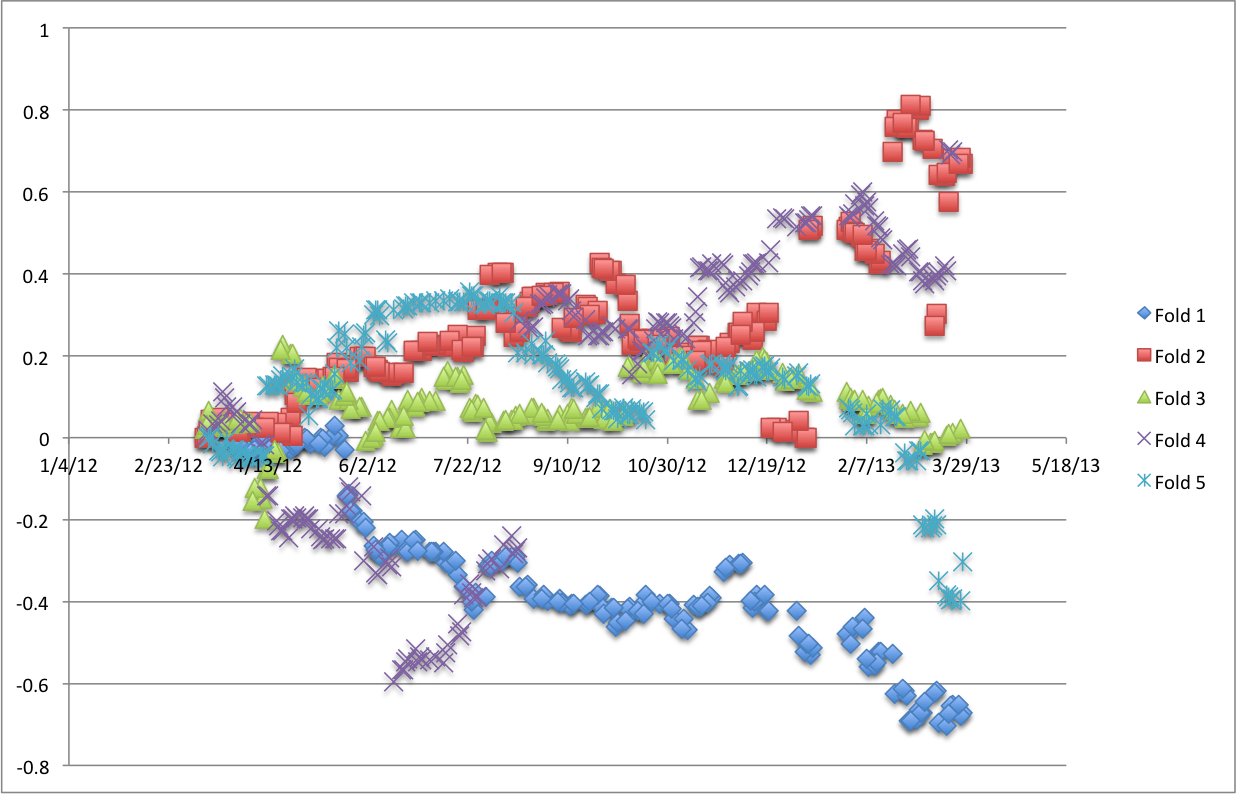
\includegraphics[width=14cm]{images/unweighted-exp-0.png}
    	\qquad
    	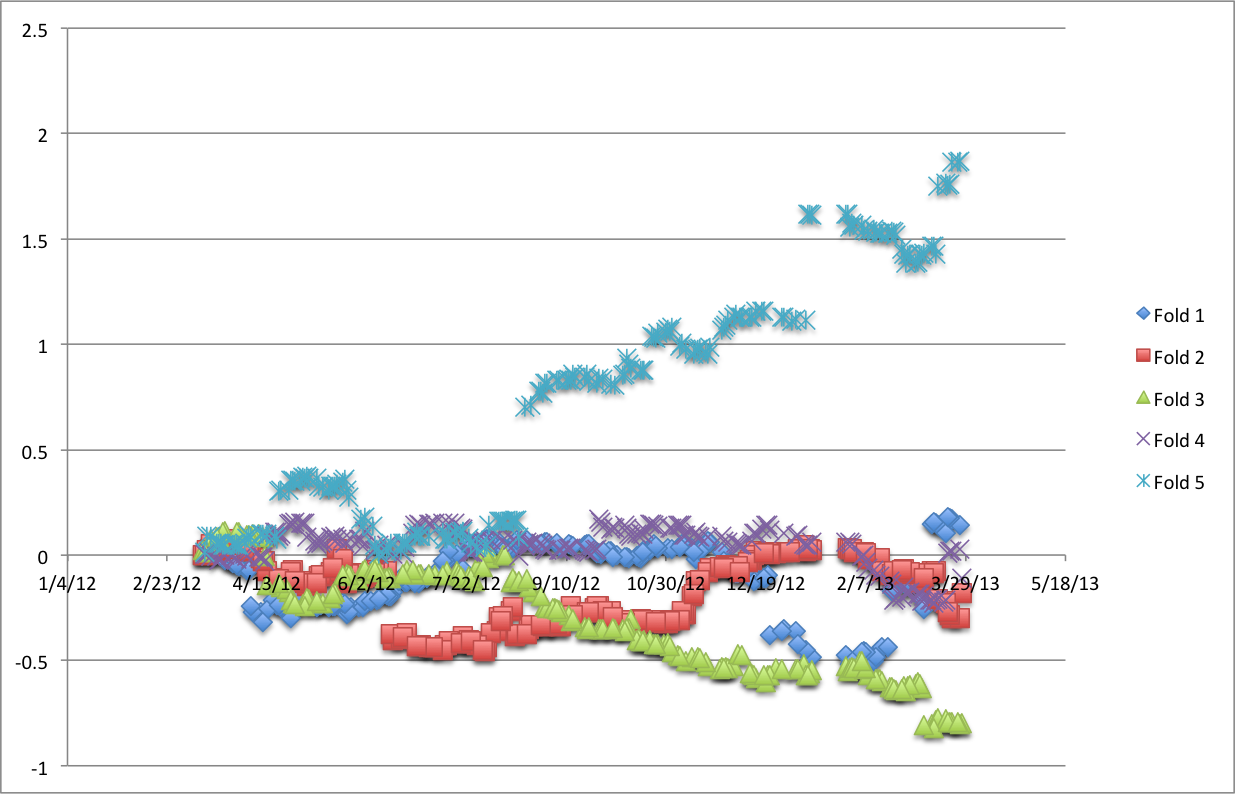
\includegraphics[width=14cm]{images/weighted-exp-0.png}
    	\caption{Segment 1 results; top: unweighted, bottom: weighted }%
    	\label{fig:1}
\end{figure}

\begin{figure}
   	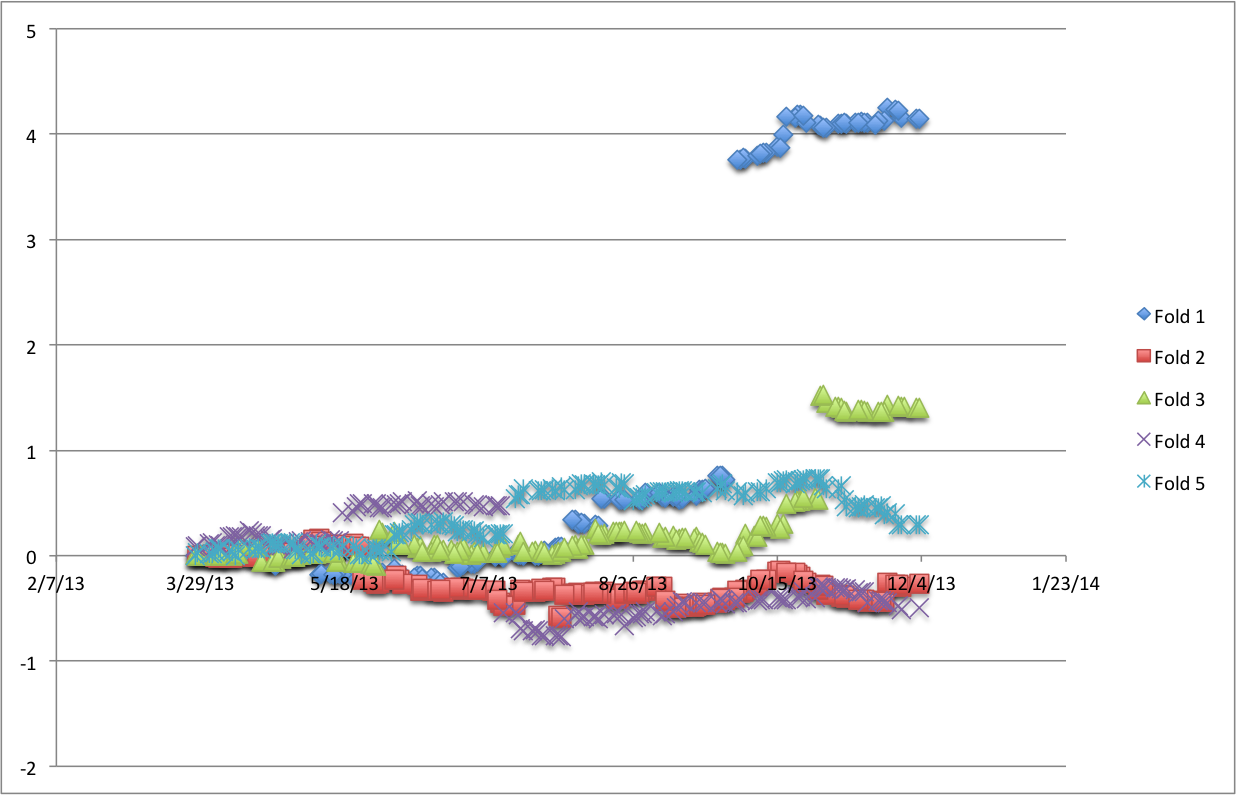
\includegraphics[width=14cm]{images/unweighted-exp-1.png}
    	\qquad
    	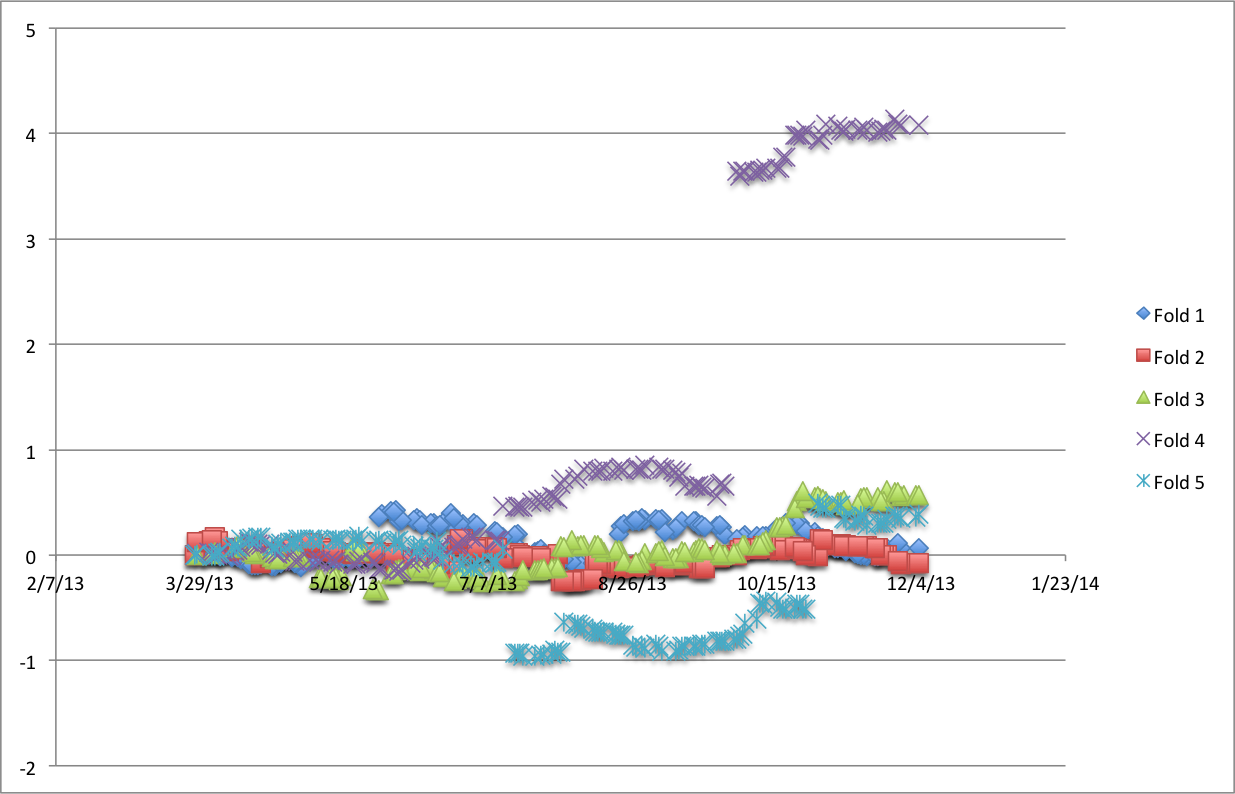
\includegraphics[width=14cm]{images/weighted-exp-1.png}
    	\caption{Segment 2 results; top: unweighted, bottom: weighted}%
    	\label{fig:2}
\end{figure}

\begin{figure}
	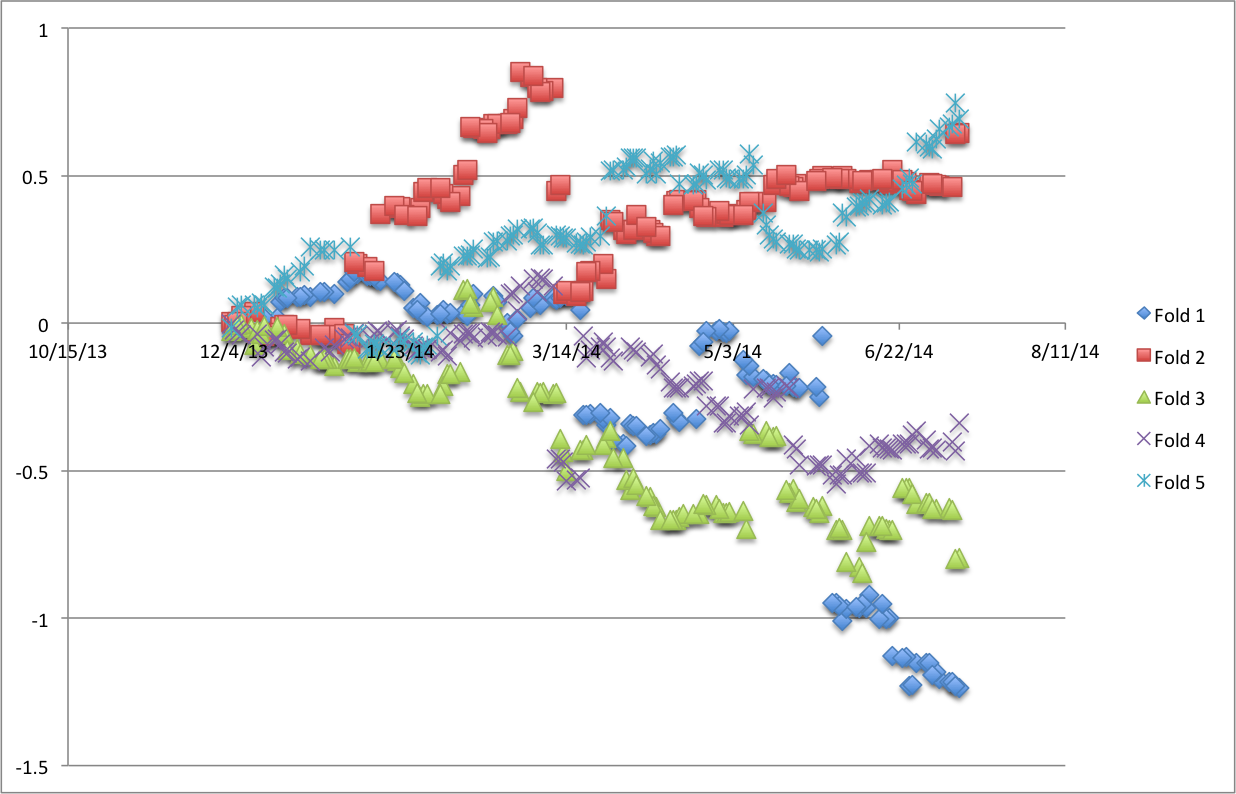
\includegraphics[width=14cm]{images/unweighted-exp-2.png}
    	\qquad
    	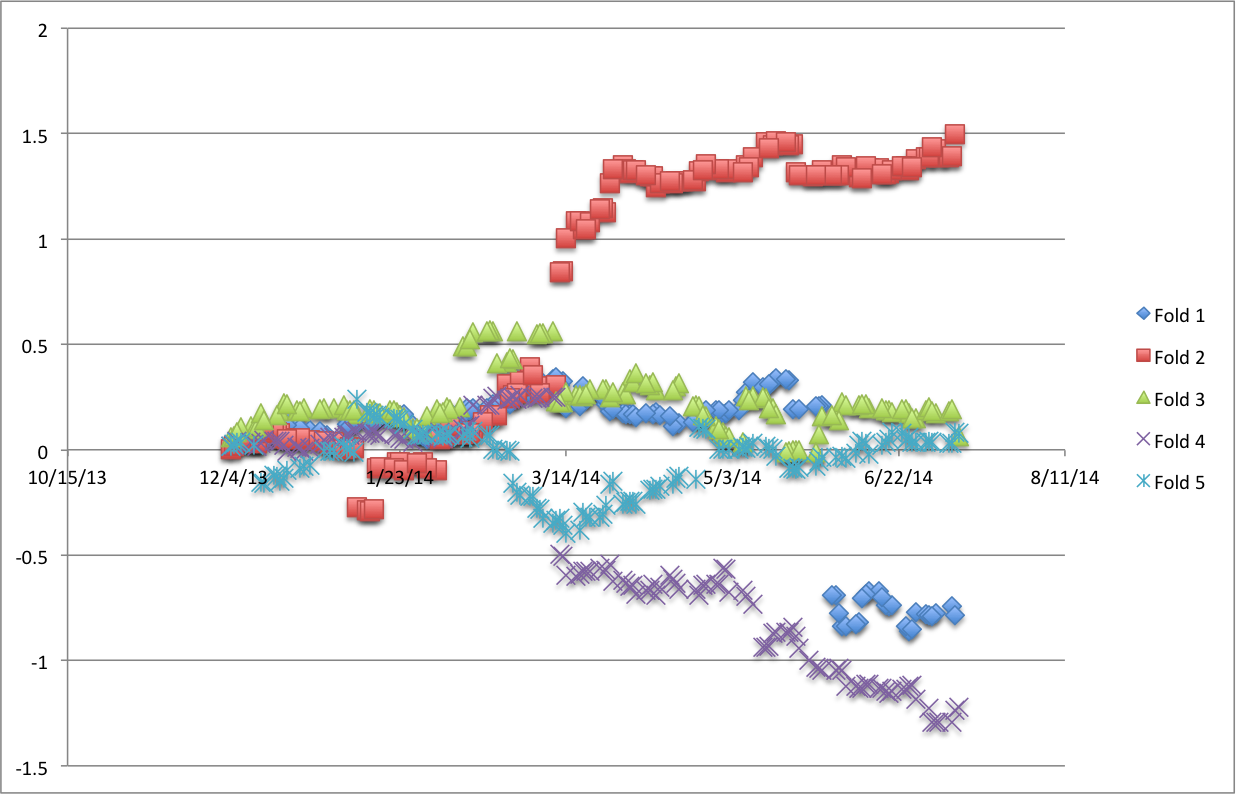
\includegraphics[width=14cm]{images/weighted-exp-2.png}
    	\caption{Segment 3 results; top: unweighted, bottom: weighted}%
    	\label{fig:3}
\end{figure}

\begin{figure}
   	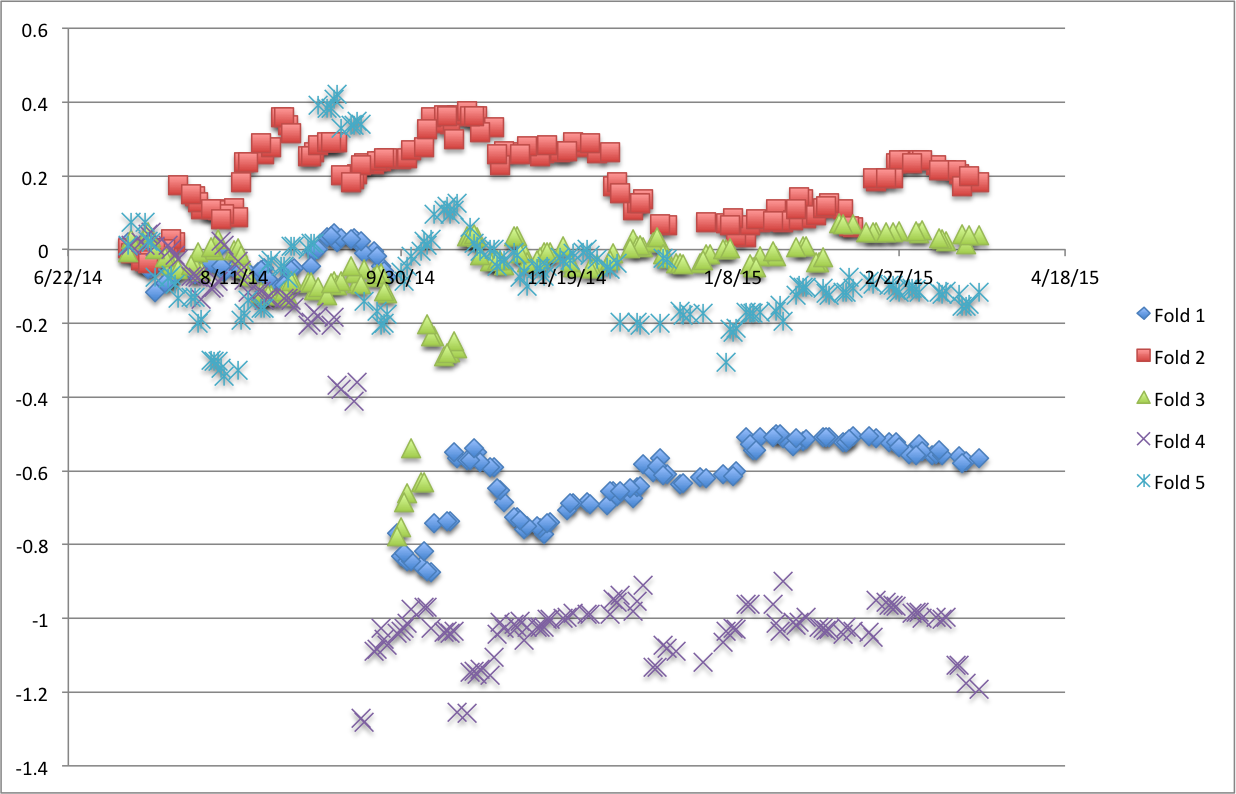
\includegraphics[width=14cm]{images/unweighted-exp-3.png}
    	\qquad
    	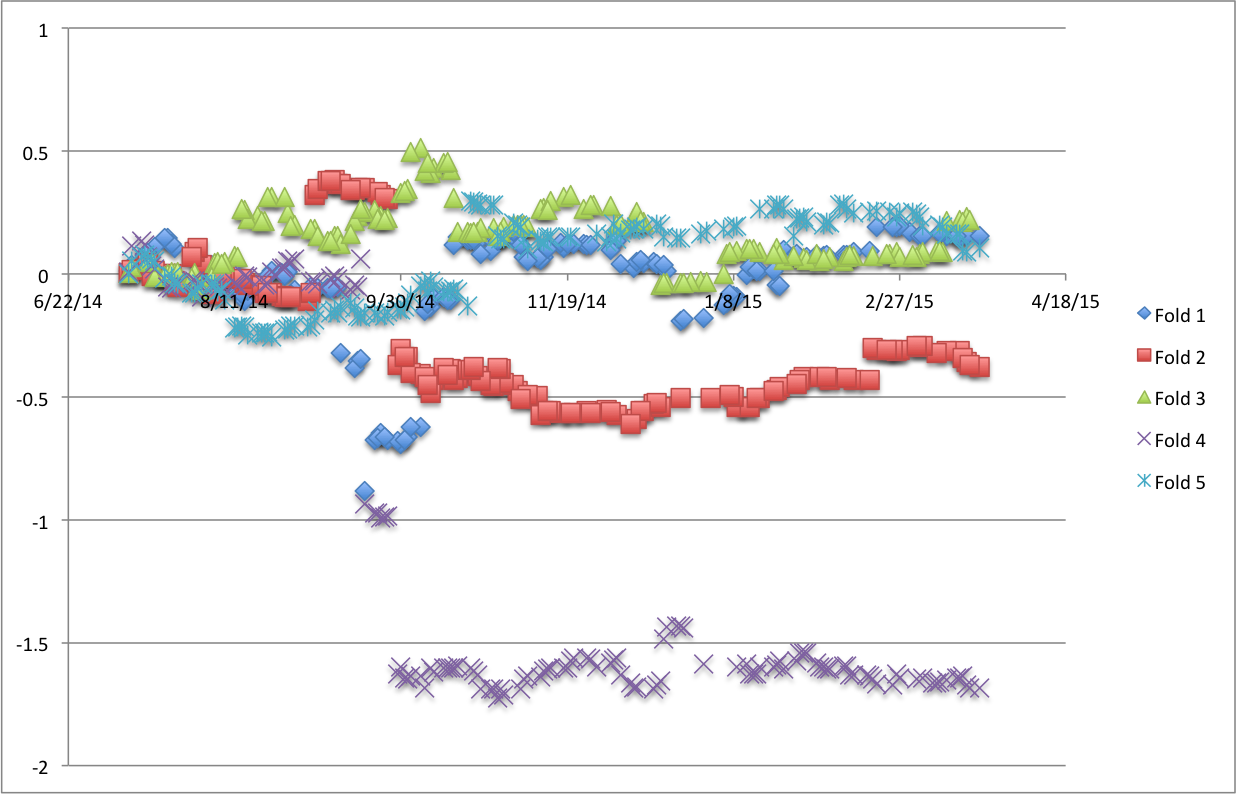
\includegraphics[width=14cm]{images/weighted-exp-3.png}
    	\caption{Segment 4 results; top: unweighted, bottom: weighted}%
    	\label{fig:4}
\end{figure}

\end{document}

%%% Local Variables:
%%% mode: latex
%%% TeX-master: t
%%% End:
